%!TEX root = ../main.tex
\chapter{Bipolartransistor}

Der Transistor ist ein Halbleiterbauelement mit dem große Leistungen am Ausgang durch kleine Signalleistungen gesteuert werden können. Diese Eigenschaft bezeichnet man als Verstärkung, da die großen Ausgangsleistungen proportional zu den kleinen Signalleistungen sind. Die für die Verstärkung erforderlichen Energie  wird einer Gleichspannungsquelle entnommen, sie liefert die Betriebsspannung $U_B$


\section{Aufbau}

Der Transistor besteht  aus drei aneinander liegenden, unterschiedlich dotierten, Halbleitergebieten. Je nach Anordnung der Gebiete werden sie in \textbf{npn-} oder \textbf{pnp- Transistoren} unterteilt.  Jedes Gebiet wird mit einem Anschluss kontaktiert. Die drei Anschlüsse bezeichnet man als \textbf{Emitter}, \textbf{Basis} und \textbf{Kollektor}.

Das Wort \textbf{Emitter} kommt aus dem lateinischen und kann mit \glqq Aussender\grqq \,  übersetzt werden. Beim Einsatz des Transistors werden aus dem Emittergebiet Ladungsträger ausgesendet. 

Der \textbf{Basisanschluss} ist der Steueranschluss. Sie ist eine Schmale Schicht zwischen dem Emitter und Kollektor und deutlich geringer Dotiert als die Emitterschicht. 

Das Wort \textbf{Kollektor} kommt ebenfalls aus dem lateinischen und kann mit dem Wort \glqq Sammler\grqq \, übersetzt werden. Der Kollektor sammelt die vom Emitter ausgesendeten Ladungsträger ein. Der Kollektor ist noch schwächer als die Basis dotiert. 

\section{Funktion eines Bipolartransistors}

Die Funktion des Bipolartransistors wird anhand des npn -Typs erklärt. Dieser findet in der Technik mehr Anwendung. Die Erklärung kann aber auf die Funktion des pnp -Transistors übertragen werden, wenn man die Richtung der Spannungs- und Strompfeile und tauscht die \glqq Elektronen\grqq \,  als \glqq Löchern\grqq betrachtet.  

Zur Vereinfachung wandeln wir den Transistor in ein Dioden-Ersatzschaltbild um. Unser Transistor besteht nun aus zwei Dioden. Eine Emitter-Basis-Diode im Eingangskreis und eine Basis-Kollektor-Diode im Ausgangskreis. (Abbildung: \ref{img: Diodeersatzschaltbild}). 

%Bild Diodenersatztschaltbild
\begin{figure}[!htb]
	\centering
	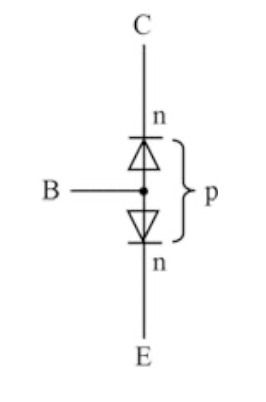
\includegraphics[scale=0.8]{images/Diodenersatzschaltbild.png} 
	\caption{Diodenersatzschaltbild \cite{Stiny2018} }
	\label{img: Diodeersatzschaltbild}
\end{figure}

Damit ein Transistor seine verstärkende und schaltende Funktionen ausüben kann, muss die Emitter-Basis-Diode in Durchlassrichtung und die Basis-Kollektor-Diode in Sperrrichutung betrieben werden. 
Als erstes wird die Emitter-Basis-Diode gesondert betrachtet (offener Ausgangskreis). Sie wird mit der Durchlassspannung $U_{BE}$ versehen, daraus resultiert der Durchlassstrom $I_E$ (Abbildung \ref{img: UBE}). Der Durchlassstrom $I_E$ setzt sich im Emittergebiet aus einer Elektronenströmung und im Basisgebiet aus einer Löcherströmung zusammen. Das Emittergebiet ist wesentlich höher dotiert als das Basisgebiet. Somit wird das Basisgebiet von Elektronen überschwemmt. Man spricht von einer \textbf{Ladungsträgerinjektion} (Abbildung \ref{img: UBE}).

\begin{figure}[!htb]
	\centering
	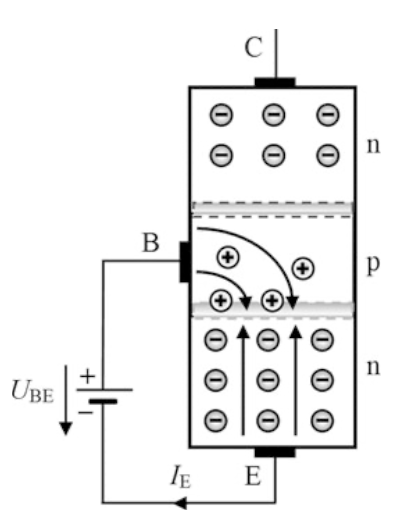
\includegraphics[scale=0.8]{images/UBEUebergang.png} 
	\caption{npn-Transistor mit angelegter Basis Emitter Spannung in Durchlassrichtung			\cite{Stiny2018}}
	\label{img: UBE}
	\end{figure}
	
	
Wird die Basis-Kollektor-Diode mit der Spannung $U_{CB}$ versehen(offener Eigangskreis) , breitet sich die Sperrschicht am pn-Übergang aus. Wichtig hierbei ist, das die Sperrschicht an Ladungsträgern verarmt, dies hat später positive Auswirkungen auf die Ladungsträgersammlung. Es fließt nur ein sehr kleiner Sperrstrom, der von den wenigen thermisch erzeugten Ladungsträger hervorgerufen wird (Abbildung \ref{img: UBC}). 	


\begin{figure}[!htb]
	\centering
	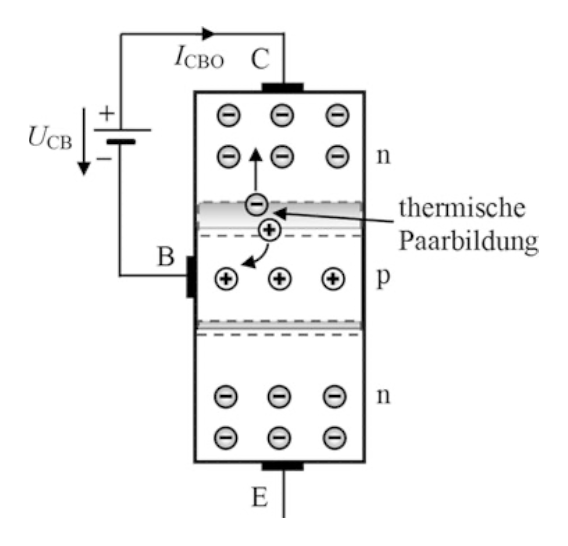
\includegraphics[scale=0.8]{images/UCEUebergang.png} 
	\caption{npn-Transistor mit angelegter Basis Kollektor Spannung in Sperrrichtung\cite{Stiny2018}}
	\label{img: UBC}		
\end{figure}	

Würden wir die Dioden in unserem Ersatzschaltbild (\ref{img: Diodeersatzschaltbild}) mit den entsprechenden Spannungen $U_{BE}$ und $U_{CB}$ versehen, würden wir nicht die Transistor typischen Eigenschaften erreichen. Es wäre kein Stromfluss zwischen Emitter und Kollektor messbar. Die einzelnen Spannungen üben keine Kräfte aufeinander aus.


In einem Transistor verfügen die beiden Dioden jedoch nur über eine gemeinsame, dünne p-Schicht. Die von dem Emitter injizierten Elektronen dringen in die gering dotierte Basisschicht ein und rekombinieren  dort teilweise mit den wenigen löchern, daraus resultiert der Basisstrom $I_B$. Aufgrund der dünnen Basisschicht werden die injizierten Elektronen vom Emitter, von dem elektrischen Feld, der Basis-Kollektor-Spannung $U_{BC}$ erfasst. Die Elektronen werden in das Kollektorgebiet gezogen und durchqueren dieses als Elektronenstrom $I_C$. Der Kollektor Strom $I_C$ ist hierbei fast so groß wie der Emitterstrom $I_E$ und deutlich größer als der Basisstrom $I_B$. Das Verhältnis zwischen Basis- und Kollektorstrom ist eine wichtige Größe zur Beschreibung eines Transistor und wird \textbf{Gleichstromverstärkungsfaktor B} genannt. 

\begin{equation}
B = \dfrac{I_C}{I_B}
\end{equation}

\begin{figure}[!htb]
	\centering
	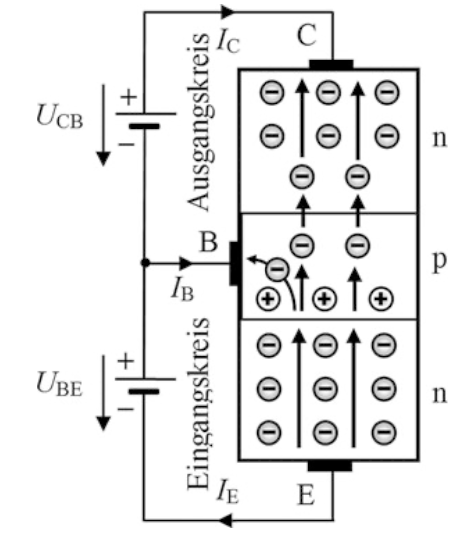
\includegraphics[scale=0.6]{images/npnTransistorDurchlass.png} 
	\caption{npn-Transistor in Durchlassrichtung \cite{Stiny2018}}
	\label{img: TransistorDurchlassrichtung}
\end{figure}

Nun lässt sich auch die Herkunft des Namens Bipolartransistor erklären. Zur Wiederholung: laut Definition werden die Elektronen im n-Gebiet als Majoritätsladungsträger bezeichnet und die Löcher als Minoritätsladungsträger. Im p-Gebiet bilden die löcher die Majoritätsladungsträger und die Elektronen die Minoritätsladungsträger. 
Die injizierten Elektronen aus der Emitterschicht stellen Minoritätsladungsträger in der Basisschicht dar. Dennoch übertreffen sie ,aufgrund der geringen Dotierung der Basisschicht, bei weitem die Anzahl der Majoritätsladungsträger der Basisschicht. 
Betrachten wir somit den gesamten Transistor setzt sich der Strom zwischen Emitter und Kollektor aus dem Majoritätsladungsträgern in der Emitterschicht, den Minoritätsladungsträgern in der Basisschicht und den Majoritätsladungsträgern aus der Kollektorschicht zusammen. Daher der Begriff  \textbf{bipolar}.




 
